\documentclass[
11pt, % The default document font size, options: 10pt, 11pt, 12pt
codirector, % Uncomment to add a codirector to the title page
]{charter}

% El títulos de la memoria, se usa en la carátula y se puede usar el cualquier lugar del documento con el comando \ttitle
\titulo{Título del proyecto}

% Nombre del posgrado, se usa en la carátula y se puede usar el cualquier lugar del documento con el comando \degreename
\posgrado{Carrera de Especialización en Sistemas Embebidos}
%\posgrado{Carrera de Especialización en Internet de las Cosas}
%\posgrado{Carrera de Especialización en Intelegencia Artificial}
%\posgrado{Maestría en Sistemas Embebidos}
%\posgrado{Maestría en Internet de las cosas}

% Tu nombre, se puede usar el cualquier lugar del documento con el comando \authorname
\autor{Nombre del Autor}

% El nombre del director y co-director, se puede usar el cualquier lugar del documento con el comando \supname y \cosupname y \pertesupname y \pertecosupname
\director{Nombre del Director}
\pertenenciaDirector{pertenencia}
% FIXME:NO IMPLEMENTADO EL CODIRECTOR ni su pertenencia
\codirector{John Doe} % para que aparezca en la portada se debe descomentar la opción codirector en el documentclass
\pertenenciaCoDirector{FIUBA}

% Nombre del cliente, quien va a aprobar los resultados del proyecto, se puede usar con el comando \clientename y \empclientename
\cliente{Nombre del cliente}
\empresaCliente{Empresa del cliente}

% Nombre y pertenencia de los jurados, se pueden usar el cualquier lugar del documento con el comando \jurunoname, \jurdosname y \jurtresname y \perteunoname, \pertedosname y \pertetresname.
\juradoUno{Nombre y Apellido (1)}
\pertenenciaJurUno{pertenencia (1)}
\juradoDos{Nombre y Apellido (2)}
\pertenenciaJurDos{pertenencia (2)}
\juradoTres{Nombre y Apellido (3)}
\pertenenciaJurTres{pertenencia (3)}

\fechaINICIO{30 de abril de 2021}		%Fecha de inicio de la cursada de GdP \fechaInicioName
\fechaFINALPlan{18 de junio de 2021} 	%Fecha de final de cursada de GdP
\fechaFINALTrabajo{15 de mayo de 2022}	%Fecha de defensa pública del trabajo final


\begin{document}

\maketitle
\thispagestyle{empty}
\pagebreak


\thispagestyle{empty}
{\setlength{\parskip}{0pt}
\tableofcontents{}
}
\pagebreak


\section*{Registros de cambios}
\label{sec:registro}


\begin{table}[ht]
\label{tab:registro}
\centering
\begin{tabularx}{\linewidth}{@{}|c|X|c|@{}}
\hline
\rowcolor[HTML]{C0C0C0}
Revisión & \multicolumn{1}{c|}{\cellcolor[HTML]{C0C0C0}Detalles de los cambios realizados} & Fecha      \\ \hline
0      & Creación del documento                                 &\fechaInicioName \\ \hline
%1      & Se completa hasta el punto 4 inclusive                 & dd/mm/aaaa \\ \hline
%2      & Se completa hasta el punto 7 inclusive
%		  Se puede agregar algo más \newline
%		  En distintas líneas \newline
%		  Así                                                    & dd/mm/aaaa \\ \hline
%3      & Se completa hasta el punto 11 inclusive                & dd/mm/aaaa \\ \hline
%4      & Se completa el plan	                                 & dd/mm/aaaa \\ \hline
\end{tabularx}
\end{table}

\pagebreak



\section*{Acta de constitución del proyecto}
\label{sec:acta}

\begin{flushright}
Buenos Aires, \fechaInicioName
\end{flushright}

\vspace{2cm}

Por medio de la presente se acuerda con el Ing. \authorname\hspace{1px} que su Trabajo Final de la \degreename\hspace{1px} se titulará ``\ttitle'', consistirá esencialmente en \textcolor{red}{la implementación de un prototipo de un sistema de control de temperatura de un calefón}, y tendrá un presupuesto preliminar estimado de \textcolor{red}{600} h de trabajo y \textcolor{red}{\$XXX}, con fecha de inicio \fechaInicioName\hspace{1px} y fecha de presentación pública \fechaFinalName.

Se adjunta a esta acta la planificación inicial.

\vfill

% Esta parte se construye sola con la información que hayan cargado en el preámbulo del documento y no debe modificarla
\begin{table}[ht]
\centering
\begin{tabular}{ccc}
\begin{tabular}[c]{@{}c@{}}Dr. Ing. Ariel Lutenberg \\ Director posgrado FIUBA\end{tabular} & \hspace{2cm} & \begin{tabular}[c]{@{}c@{}}\clientename \\ \empclientename \end{tabular} \vspace{2.5cm} \\
\multicolumn{3}{c}{\begin{tabular}[c]{@{}c@{}} \supname \\ Director del Trabajo Final\end{tabular}} \vspace{2.5cm} \\
%\begin{tabular}[c]{@{}c@{}}\jurunoname \\ Jurado del Trabajo Final\end{tabular}     &  & \begin{tabular}[c]{@{}c@{}}\jurdosname\\ Jurado del Trabajo Final\end{tabular}  \vspace{2.5cm}  \\
%\multicolumn{3}{c}{\begin{tabular}[c]{@{}c@{}} \jurtresname\\ Jurado del Trabajo Final\end{tabular}} \vspace{.5cm}
\end{tabular}
\end{table}

\section{1. Descripción técnica-conceptual del proyecto a realizar}
\label{sec:descripcion}

Para productos de ámbitos espaciales, como lo son los satélites, muchas veces es difícil, y en ocasiones imposible, generar escenarios realistas para pruebas de los elementos que los componen. Ya sea por no poder generar las mismas condiciones ambientales, o porque la naturaleza de la maniobra que se busca probar implicaría un daño a los equipos bajo revisión.

En este contexto, es común replicar los elementos de interés de manera programada, cumpliendo con cierto grado de representación. De manera tal que se comporten de la manera más similar posible a su contraparte física. Estos elementos, íntegramente desarrollados en software, se los llaman emulados o simulados. Uno de los componentes que se suele tener mayor interés en simular es el procesador de la computadora a bordo.

El término Computadora a Bordo (OBC, por las siglas en inglés de On Board Computer) suele referirse a la unidad en la que se ejecuta el Software A Bordo (OBSW, por sus siglas en inglés de On Board Software) y su rol principal es el control de los subsistemas del satélite. Esto incluye recolectar información de diferentes subsistemas, analizarla y tomar las decisiones y acciones apropiadas cuando sea requerido.

El foco principal de este trabajo es el microprocesador contenido en la OBC. Cabe destacar, que hoy en día existen emuladores tanto de código abierto como privativos para distintos microprocesadores. Un ejemplo claro de emulador de código abierto es Qemu, que abarca un amplio abanico de microprocesadores, entre ellos, algunos utilizables en el ámbito espacial.

En el contexto de los emuladores, cada uno aborda el problema en cuestión, pero conlleva sus propias desventajas. Por ejemplo, en el caso de emuladores como Qemu, diseñados para ser genéricos, pueden requerir un esfuerzo adicional para adaptarlos a un procesador específico, como es el GR712RC. Esto se debe a que la flexibilidad genérica puede implicar una pérdida de rendimiento o la necesidad de familiarizarse con su API.

Por otro lado, los emuladores comerciales suelen estar optimizados para procesadores específicos, lo que puede brindar un excelente rendimiento en esas circunstancias particulares. Sin embargo, estos emuladores pueden ser limitados en cuanto a su capacidad de personalización, instrumentación y capacidad de integración, lo que puede dificultar su adaptación a necesidades específicas o la depuración de software en entornos no nominales.

Bajo estas premisas se plantea crear un emulador de microprocesador Leon3 para desarrollo de software satelital y simuladores. En la figura \ref{fig:Components} se deja en evidencia un diagrama de bloques del hardware que se busca replicar. Al ser un desarrollo a medida, se tendrá la ventaja de la no-diversificación del procesador, es decir, estará únicamente orientado a un solo microprocesador. Esperando una ganancia en performance comparado con su contraparte de código abierto. Al mismo tiempo, se tendrá un conocimiento extenso del alcance y limitaciones de las capacidades del software en cuestión. Haciendo, de esta manera, más simple la integración y depuración en su uso.

\begin{figure}[htpb]
\centering
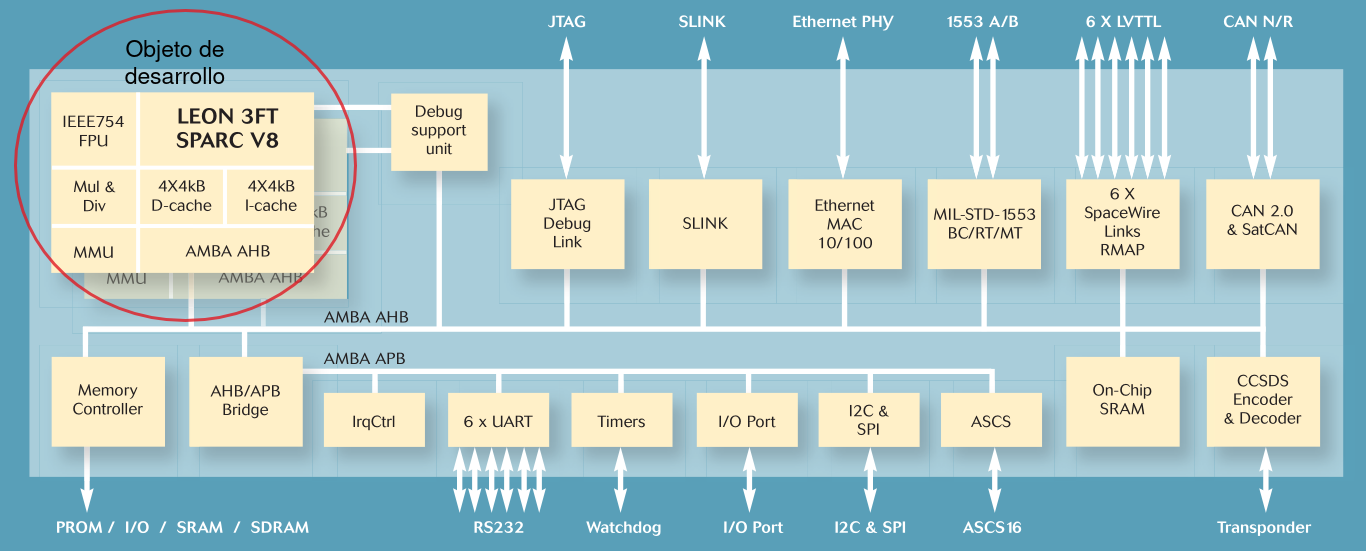
\includegraphics[width=1\textwidth]{./assets/Components.png}
\caption{Diagrama en bloques del sistema.}
\label{fig:Components}
\end{figure}

\vspace{25px}

\newpage

Para lograr el objetivo descrito, se ha decidido utilizar el framework LLVM. Este se empleará para generar el conjunto de instrucciones admitido por el microprocesador Leon3. La elección de LLVM se fundamenta en varios factores clave que hacen de esta plataforma una opción sólida y versátil. Tales como que cuenta con una comunidad de desarrollo activa y comprometida, lo que garantiza un soporte continuo y actualizaciones regulares que son esenciales para mantener la robustez y eficiencia del sistema. También, al poseer soporte nativo con Leon3, es una fuente de análisis y guía en los casos donde los manuales no sean lo suficientemente claros.

Por último, es importante subrayar que el presente trabajo no se iniciará desde cero, sino que se aprovechará una base de código preexistente gentilmente proporcionada por el director de tesis. Esta base no solo servirá como una hoja de guía para el proceso de desarrollo, sino que también desempeñará un papel clave en la aceleración de todo el proyecto.


\section{2. Identificación y análisis de los interesados}
\label{sec:interesados}

\begin{table}[ht]
%\caption{Identificación de los interesados}
%\label{tab:interesados}
\begin{tabularx}{\linewidth}{@{}|l|X|X|l|@{}}
\hline
\rowcolor[HTML]{C0C0C0}
Rol           & Nombre y Apellido & Organización 	 & Puesto 	\\ \hline
Cliente       & Lic. \clientename      &\empclientename &   Especialista Tecnológico     	\\ \hline
Responsable   & \authorname       & FIUBA        	 & Alumno 	\\ \hline
Orientador    & Esp. Lic. \supname	        & \pertesupname  & Director Trabajo final \\ \hline
Usuario final    & Departamento de Embebidos y Sistemas Críticos & \pertesupname  & - \\ \hline
\end{tabularx}
\end{table}

\begin{itemize}
\item Cliente: Lic. Matías Pinedo, del Departamento de Embebidos y Sistemas Críticos de la empresa INVAP S.E., quien aporta su visión y experiencia necesaria para desarrollar el proyecto.
\item Orientador: es el director del trabajo final, quien aportará sus conocimientos técnicos y experiencia para la realización del proyecto.
\item Usuario final: será el Departamento de Embebidos y Sistemas Críticos de la empresa INVAP S.E.
\end{itemize}

%% \end{consigna} % este comando se debe borrar para la entrega, junto con la contraparte \begin{consigna}{red}



\section{3. Propósito del proyecto}
\label{sec:proposito}

El propósito de este proyecto es desarrollar un emulador para ejecución de software de vuelo para microprocesadores de la familia Leon3 utilizando el framework LLVM a partir de un código preexistente provisto.


\section{4. Alcance del proyecto}
\label{sec:alcance}

El presente trabajo incluye:

\begin{itemize}
\item El desarrollo del software de emulación.
\item Una API para su uso en el lenguaje de programación C.
\item El desarrollo de un sistema de depuración para una ejecución.
\end{itemize}

El proyecto no incluye:

\begin{itemize}
\item Desarrollo de software para el procesador Leon3 representativo con el uso que se le piense dar.
\item Librerías utilitarías para generación de código fuente.
\item Emulación completa sobre todos periféricos asociados.
\end{itemize}



\section{5. Supuestos del proyecto}
\label{sec:supuestos}

Para el desarrollo del presente proyecto se supone que:

\begin{itemize}
\item La empresa va a proveer de un modelo de referencia (físico o emulado) para la realización del proyecto.
\item El proyecto puede ser realizado sin necesidad de hacer pruebas en campo.
\item Se contará con soporte y apoyo por parte de expertos de la empresa.
\item El proyecto puede ser realizado sin necesidad de ir a las oficinas de la empresa.
\end{itemize}


\section{6. Requerimientos}
\label{sec:6-requerimientos}

\begin{enumerate}
\item Requerimientos funcionales
	\begin{enumerate}
  \item El emulador deberá poder cargar y ejecutar binarios valídos para Leon3, tales como los que se cargarían al hardware real.
	\item Deberá poder ejecutarse en Linux.
  \item Se deberá desarrollar un ambiente de automatización de pruebas en Gitlab CI.
  \item Se deberán desarrollar tests unitarios que verifiquen parte de set de instrucciones del emulador.
  \item Se deberá poder utilizar el software como librería compartida.
	\end{enumerate}

\item Requerimientos de documentación
	\begin{enumerate}
	\item La API que será expuesta como librería deberá estár documentada con Doxygen.
	\item Se realizará un manual de usuario que describa los funcionamientos clave del software.
	\end{enumerate}

\item Requerimientos de desarrollo de software
  \begin{enumerate}
  \item El software deberá ser escrito en C++.
  \item La API expuesta deberá ser en C.
  \item El software debe mantenerse bajo control de versiones en Gitlab.
  \end{enumerate}
\end{enumerate}



\section{7. Historias de usuarios (\textit{Product backlog})}
\label{sec:7-historias-de-usuarios-product-backlog}


Roles:

\begin{itemize}
\item Desarrollador de modelos simulados: quien se encarga de desarrollar dispositivos de manera simulada. Tales como podrían ser memorias, FPGAs y/o periféricos.
\item Desarrollador de software de vuelo: quien se encarga de desarrollar un driver o software que usa interfaces de bajo nivel. Durante el diseño e implementación, utiliza este sistema para interactuar con el hardware.
\item Ingeniero de pruebas: quien se encarga de automatizar los ensayos de calificación de hardware y/o de componentes que lo emulen.
\end{itemize}

Story Points:

\begin{itemize}
\item Se analizarán las historias según dificultad, complejidad e incertidumbre, tomando valores de Fibonacci usando el siguiente criterio:
  \begin{enumerate}
  \item Dificultad: cantidad de trabajo a realizar. Representado con la letra ``\textbf{D}''.

	  \begin{itemize}
	  \item Bajo: 1
	  \item Medio: 3
	  \item Alto: 13
	  \end{itemize}

  \item Complejidad: complejidad de trabajo a realizar. Representado con la letra ``\textbf{C}''.

	  \begin{itemize}
	  \item Bajo: 1
	  \item Medio: 5
	  \item Alto: 13
	  \end{itemize}

  \item Incertidumbre: riesgo del trabajo a realizar. Representado con la letra ``\textbf{I}''.

	  \begin{itemize}
	  \item Bajo: 1
	  \item Medio: 3
	  \item Alto: 5
	  \end{itemize}

  \end{enumerate}

\end{itemize}

Historias de Usuarios:

\begin{itemize}
\item Como desarrollador de modelos simulados quiero poder comunicarme con el software de vuelo para verificar el correcto functionamiento de mi desarrollo. D: 3, C: 5, I: 5 Total = 13p.

\item Como desarrollador de modelos simulados quiero poder ejecutar el software de vuelo como una biblioteca para evitar posibles desfasajes entre componentes. D: 3, C: 1, I: 1. Total = 5p.

\item Como desarrollador de software de vuelo quiero poder estimular los registros, memorias y hardware para el desarrollo de controladores (\textit{drivers}). D: 13, C: 13, I: 5. Total = 34p.

\item Como desarrollador de software de vuelo quiero que mi software corra a tiempo real para que las emulaciones sean representativas. D: 5, C: 5, I: 5. Total = 21p.

\item Como ingeniero de pruebas quiero que mis pruebas puedan ser ejecutadas automáticamente en un entonces de desarrollo continuo (por ejemplo GitLab CI) para ahorrar tiempo y evitar errores humanos. D: 3, C: 2, I: 2. Total = 8p.
\end{itemize}


\section{8. Entregables principales del proyecto}
\label{sec:8-entregables-principales-del-proyecto}

Los entregables del proyecto son:

\begin{itemize}
	\item Librería de emulación con sus respectivos headers.
	\item Documentación Doxygen de la API.
	\item Manual de uso.
\end{itemize}



\section{9. Desglose del trabajo en tareas}
\label{sec:9-desglose-del-trabajo-en-tareas}


\begin{enumerate}
\item Gestión del proyecto (24 h):
  \begin{enumerate}
  \item Definición de requerimientos con el cliente (4 h).
  \item Planificación (20 h).
  \end{enumerate}

\item Investigación y capacitación en la arquitectura del microprocesador (33 h):

  \begin{enumerate}
  \item Recopilación de documentación online (3 h).
  \item Lectura y comprensión de los documentos (10 h).
  \item Capacitación sobre el conjunto de instrucciones del procesador (20 h).
  \end{enumerate}

\item Desarrollo del ambiente de automatización (16 h):

  \begin{enumerate}
  \item Creación del repositorio de desarrollo (2 h).
  \item Creación del ambiente de CI/CD para tests (4 h).
  \item Desarrollo  del ambiente CI/CD para documentación (6 h).
  \item Creación del ambiente de CI/CD para empaquetado (4 h).
  \end{enumerate}

\item Internalización de código pre-existente (46 h):

  \begin{enumerate}
  \item Revisión y análisis del código existente (12 h).
  \item Selección del código a reutilizar e importación (30 h).
  \item Refactorización del código (4 h).
  \end{enumerate}

\item Investigación y capacitación en el framework de LLVM (50 h):

  \begin{enumerate}
  \item Lectura de documentación (20 h).
  \item Internalización con su API (20 h).
  \item Pruebas de límites y alcances del framework (10 h).
  \end{enumerate}

\item Desarrollo del software (180 h):

  \begin{enumerate}
  \item Desarrollo de modelos de periféricos (40 h).
  \item Desarrollo de modelos de memorias y registros (30 h).
  \item Desarrollo de instrucciones. Se estima funcionalidad mínima de un subset de instrucciones, calculando 1 hora por instrucción. (110 h).
    \begin{enumerate}
    \item Desarrollo de instrucciones aritméticas y lógicas (40 h).
    \item Desarrollo de instrucciones de carga y descarga de memoria (40 h).
    \item Desarrollo de instrucctiones escritura/lectura de registros de control (30 h).
    \end{enumerate}
  \end{enumerate}

\item Desarrollo de tests unitarios y de API (90 h):

  \begin{enumerate}
  \item Pruebas unitarias de modelos (20 h).
  \item Pruebas unitarias de instrucciones (40 h).
  \item Pruebas de API (20 h).
  \item Corrección de errores (10 h).
  \end{enumerate}

\item Documentación (50 h):

  \begin{enumerate}
  \item Creación del manual de usuario (40 h).
  \item Documentación de API en Doxygen (10 h).
  \end{enumerate}

\item Presentación del trabajo (112 h):

  \begin{enumerate}
  \item Recopilación de datos de ensayos y organización de resultados para las
    memorias (40 h).
  \item Redacción de las memorias (40 h).
  \item Presentación del trabajo (32 h).
  \end{enumerate}
\end{enumerate}

Cantidad total de horas: 621 horas.


\section{10. Diagrama de Activity On Node}
\label{sec:AoN}

En la figura \ref{fig:AoN} se ilustra el diagrama de \textit{Activity on Node}. Las tareas están agrupadas en la misma forma que en la sección anterior:

\begin{enumerate}
\item Gestión del proyecto.
\item Investigación y capacitación en la arquitectura del microprocesador.
\item Desarrollo del ambiente de automatización.
\item Internalización de código pre-existente.
\item Investigación y capacitación en el framework de LLVM.
\item Desarrollo del software.
\item Desarrollo de tests unitarios y de API.
\item Documentación.
\item Presentación del trabajo.
\end{enumerate}

Cada tarea está etiquetada con una letra \textbf{T} seguida de su número de tarea. Por ejemplo, T1.1 corresponde a la tarea ``1.1 - Definición de requerimientos con el cliente''. El camino crítico, cuya duración es de 382 horas, se muestra resaltado en color rojo. El camino semicrítico se muestra resaltado en color azul. Mientras que el no crítico en se denota con una flecha puntuada.

\begin{figure}[htpb]
  \centering
  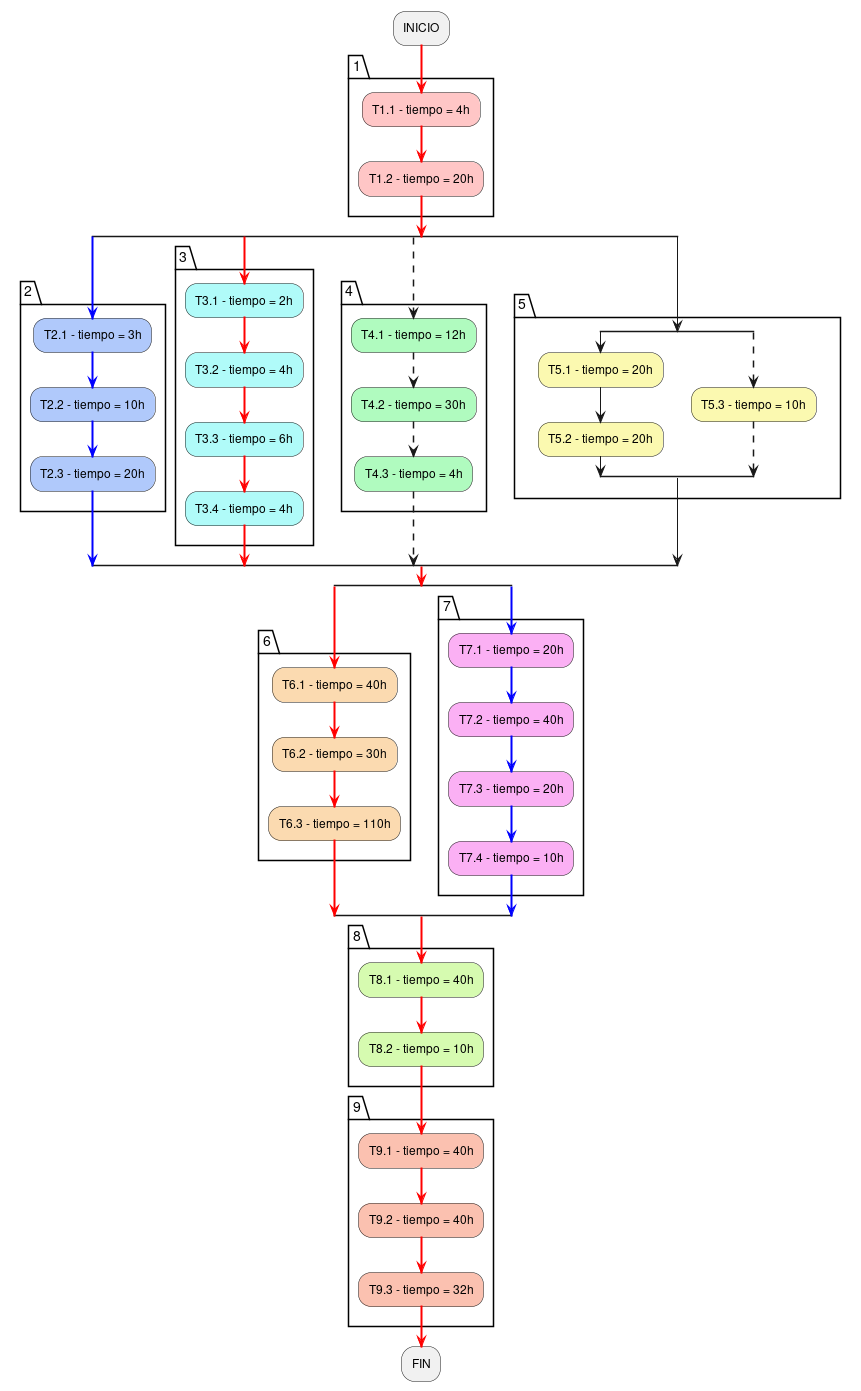
\includegraphics[width=.90\textwidth]{./assets/AoN.png}
  \caption{Diagrama de \textit{Activity on Node}.}
  \label{fig:AoN}
\end{figure}

\vspace{25px}



\section{11. Diagrama de Gantt}
\label{sec:gantt}

Debido a que todas las tareas serán realizadas por el responsable del proyecto (es decir, una sola persona) las dependencias de las actividades del diagrama de \textit{Activity on Node} fueron adaptadas para reflejar la imposibilidad de ejecutar tareas en paralelo.

El diagrama de Gantt se muestra separado en dos partes. Un cuadro \ref{tab:wbs} que contiene el desglose de tareas y la figura \ref{fig:Gantt} que contiene el diagrama propiamente dicho.

\begin{table}[ht]
  \centering

  \begin{tabularx}{\linewidth}{@{}|c|X|c|c|@{}}
    \hline
    \rowcolor[HTML]{C0C0C0}
    WBS & \multicolumn{1}{c|}{\cellcolor[HTML]{C0C0C0}Nombre} & Inicio  & Fin     \\ \hline
    1.1 & Definición de requerimientos con el cliente & 01/08/23 & 01/08/23 \\ \hline
    1.2 & Planificación & 03/08/23 & 12/08/23 \\ \hline
    2.1 & Recopilación de documentación online & 13/08/23 & 14/08/23\\ \hline
    2.2 & Lectura y comprensión de los documentos & 15/08/23 & 19/08/23\\ \hline
    2.3 & Capacitación sobre el conjunto de instrucciones del procesador & 20/08/23 & 29/08/23\\ \hline
    3.1 & Creación del repositorio de desarrollo & 30/08/23 & 30/08/23\\ \hline
    3.2 & Creación del ambiente de CI/CD para tests & 31/08/23 & 01/09/23\\ \hline
    3.3 & Desarrollo  del ambiente CI/CD para documentación & 02/09/23 & 04/09/23\\ \hline
    3.4 & Creación del ambiente de CI/CD para empaquetado & 05/09/23 & 06/09/23\\ \hline
    4.1 & Revisión y análisis de código existente & 07/09/23 & 12/09/23\\ \hline
    4.2 & Selección del código a reutilizar e importación & 13/09/23 & 25/09/23\\ \hline
    4.3 & Refactorización del código & 27/09/23 & 28/09/23\\ \hline
    5.1 & Lectura de documentación & 29/09/23 & 08/10/23\\ \hline
    5.2 & Internalización con su API & 09/10/23 & 18/10/23\\ \hline
    5.3 & Pruebas de límites y alcances del framework & 19/10/23 & 23/10/23\\ \hline
    6.1 & Desarrollo de modelos de periféricos & 24/10/23 & 11/11/23\\ \hline
    6.2 & Desarrollo de modelos de memorias y registros & 12/11/23 & 25/11/23\\ \hline
    6.3 & Desarrollo de instrucciones & 26/11/23 & 16/01/24\\ \hline
    7.1 & Pruebas unitarias de modelos & 17/01/24 & 26/01/24\\ \hline
    7.2 & Pruebas unitarias de instrucciones & 27/01/24 & 14/02/24\\ \hline
    7.3 & Pruebas de API & 15/02/24 & 24/02/24\\ \hline
    7.4 & Corrección de errores & 25/02/24 & 29/02/24\\ \hline
    8.1 & Creación del manual de usuario & 01/03/24 & 19/03/24\\ \hline
    8.2 & Documentación de API en Doxygen & 20/03/24 & 24/03/24\\ \hline
    9.1 & Preparación de las memorias & 25/03/24 & 12/04/24\\ \hline
    9.2 & Redacción de las memorias & 13/04/24 & 01/05/24\\ \hline
    9.3 & Presentación del trabajo & 02/05/24 & 16/05/24\\ \hline
  \end{tabularx}
  \caption{Desglose de tareas.}
  \label{tab:wbs}
\end{table}


\begin{landscape}

  \begin{figure}[htpb]
    \centering
    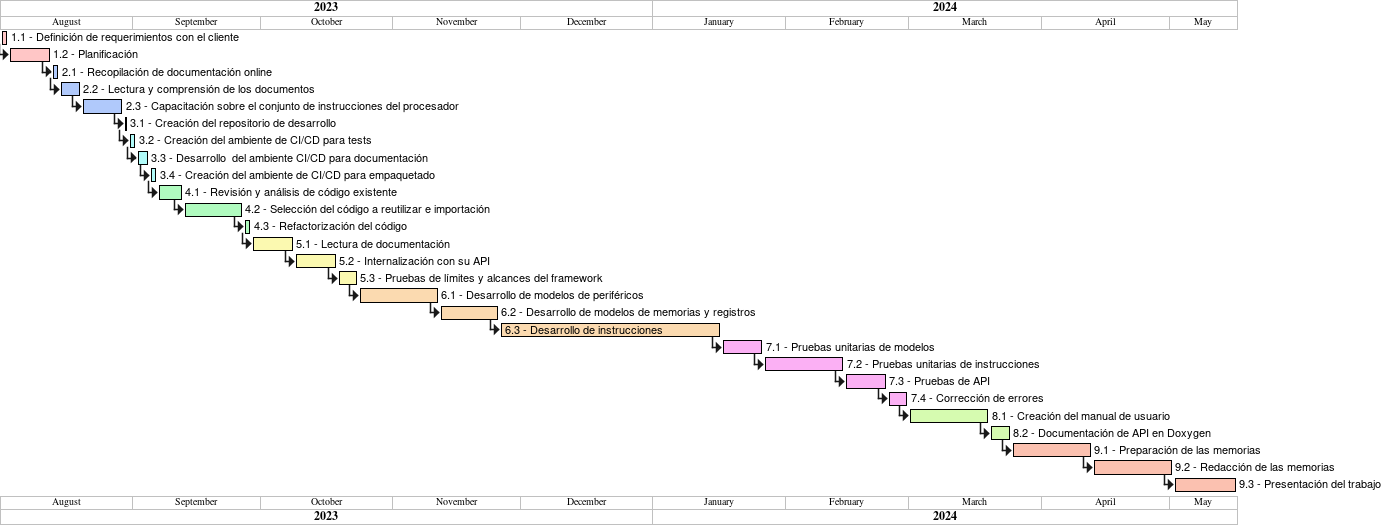
\includegraphics[width=1.5\textwidth]{./assets/Gantt.png}
    \caption{Diagrama de Gantt.}
    \label{fig:Gantt}
  \end{figure}

  \vspace{25px}


\end{landscape}


\section{12. Presupuesto detallado del proyecto}
\label{sec:presupuesto}

A continuación se presenta el presupuesto detallado del proyecto expresado en dólares americanos:

\begin{table}[htpb]
  \centering
  \begin{tabularx}{\linewidth}{@{}|X|c|r|r|@{}}
    \hline
    \rowcolor[HTML]{C0C0C0}
    \multicolumn{4}{|c|}{\cellcolor[HTML]{C0C0C0}COSTOS DIRECTOS} \\ \hline
    \rowcolor[HTML]{C0C0C0}
    Descripción &
    \multicolumn{1}{c|}{\cellcolor[HTML]{C0C0C0}Cantidad} &
    \multicolumn{1}{c|}{\cellcolor[HTML]{C0C0C0}Valor unitario} &
    \multicolumn{1}{c|}{\cellcolor[HTML]{C0C0C0}Valor total} \\ \hline
    Horas del responsable &
    \multicolumn{1}{c|}{621} &
    \multicolumn{1}{c|}{US\textdollar 30} &
    \multicolumn{1}{c|}{US\textdollar 18.630 } \\ \hline
    Computadora &
    \multicolumn{1}{c|}{1} &
    \multicolumn{1}{c|}{US\textdollar 600} &
    \multicolumn{1}{c|}{US\textdollar 600} \\ \hline
    \multicolumn{1}{|l|}{Gastos operativos. (oficina, servicios, etc.)} &
    10 &
    \multicolumn{1}{c|}{US\textdollar 5 } &
    \multicolumn{1}{c|}{US\textdollar 50 }
    \\ \hline
    \multicolumn{3}{|c|}{SUBTOTAL} &
    \multicolumn{1}{c|}{US\textdollar 19.280} \\ \hline
    \rowcolor[HTML]{C0C0C0}
    \multicolumn{4}{|c|}{\cellcolor[HTML]{C0C0C0}COSTOS INDIRECTOS} \\ \hline
    \rowcolor[HTML]{C0C0C0}
    Descripción &
    \multicolumn{1}{c|}{\cellcolor[HTML]{C0C0C0}Cantidad} &
    \multicolumn{1}{c|}{\cellcolor[HTML]{C0C0C0}Valor unitario} &
    \multicolumn{1}{c|}{\cellcolor[HTML]{C0C0C0}Valor total} \\ \hline
    \multicolumn{1}{|l|}{Modelo de referencia (físico o emulado)} &
    1 &
    X (*) & X (*)
    \\ \hline
    \multicolumn{3}{|c|}{SUBTOTAL} &
    \multicolumn{1}{c|}{-} \\ \hline
    \rowcolor[HTML]{C0C0C0}
    \multicolumn{3}{|c|}{TOTAL} & US\textdollar 19.280
    \\ \hline
  \end{tabularx}%
\end{table}

(*) Valor confidencial.



\section{13. Gestión de riesgos}
\label{sec:riesgos}

\begin{enumerate}[label=\alph*)] % Lowercase alphabetic enumeration
\item Identificación de los riesgos y estimación de sus consecuencias:

  A continuación se detallan cinco posibles riesgos inherentes al proyecto. Los mismos son evaluados según su grado de severidad y su probabilidad de ocurrrencia tomando valores del 1 (bajo) al 10 (alto).

  %%%%%%%%%%%%%%%%%%%%%%%%%%%%%%%%%%%%%%%%%%%%%%%%%%%%%%%%%%%%%%%%%%%%%
  \textbf{Riesgo 1}: no finalizar el proyecto en el plazo de tiempo establecido.

  \begin{itemize}
  \item Severidad (S): 10. Severidad alta porque no se cumpliría con la fecha de entrega límite establecida.
  \item Ocurrecia (O): 6. Es probable ya que la totalidad del proyecto se realizará fuera del horario laboral.
  \end{itemize}

  %%%%%%%%%%%%%%%%%%%%%%%%%%%%%%%%%%%%%%%%%%%%%%%%%%%%%%%%%%%%%%%%%%%%%
  \textbf{Riesgo 2}: dificultad en la capacitación en el \textit{framework} LLVM.


  \begin{itemize}
  \item Severidad (S): 8. Severidad media/alta porque se planea tomar varias funcionalidad de dicho \textit{framework}, que de otra manera implicarían un esfuerzo mucho mayor.
  \item Ocurrecia (O): 5. Es probable que suceda ya que es un proyecto de alta complejidad, pero al mismo tiempo tiene mucha documentación asociada.
  \end{itemize}

  %%%%%%%%%%%%%%%%%%%%%%%%%%%%%%%%%%%%%%%%%%%%%%%%%%%%%%%%%%%%%%%%%%%%%
  \textbf{Riesgo 3}: bajo desempeño del emulador, con ejecuciones que no alcancen al tiempo real.

  \begin{itemize}
  \item Severidad (S): 3. Baja severidad, ya que se plantea un prototipo sin funcionanlidad completa, que luego podría ser optimizado para cumplir los requerimientos de performance.
  \item Ocurrecia (O): 6. Es probable que suceda ya que se trata de un \textit{software} de alta complejidad computacional.
  \end{itemize}

  %%%%%%%%%%%%%%%%%%%%%%%%%%%%%%%%%%%%%%%%%%%%%%%%%%%%%%%%%%%%%%%%%%%%%
  \textbf{Riesgo 4}: dificultad en la comprensión de documentos, tanto de \textit{datasheets} como de manuales de arquitectura del procesador.


  \begin{itemize}
  \item Severidad (S): 10. Alta severidad, ya que sin entender dichos documentos no es posible desarrollar software que cumpla el correcto funcionamiento del procesador.
  \item Ocurrecia (O): 8. Se estima una alta probabilidad de ocurrencia debido a que son documentos sumamente extensos y de gran detalle técnico.
  \end{itemize}

  %%%%%%%%%%%%%%%%%%%%%%%%%%%%%%%%%%%%%%%%%%%%%%%%%%%%%%%%%%%%%%%%%%%%%
  \textbf{Riesgo 5}: dificultad para localizar y depurar errores de desarrollo del \textit{software}.


  \begin{itemize}
  \item Severidad (S): 4. Media severidad, ya que al estár internalizado con el código fuente, todas las fuentes de errores son facilmente identificables.
  \item Ocurrecia (O): 8. Media/alta ocurrencia, ya que es normal cometer errores en la programación de código.
  \end{itemize}

  %%%%%%%%%%%%%%%%%%%%%%%%%%%%%%%%%%%%%%%%%%%%%%%%%%%%%%%%%%%%%%%%%%%%%

\item Tabla de gestión de riesgos: (El RPN se calcula como RPN = $\text{S} \times \text{O}$)


  \begin{table}[htpb]
    \centering
    \begin{tabularx}{\linewidth}{@{}|X|c|c|c|c|c|c|@{}}
      \hline
      \rowcolor[HTML]{C0C0C0}
      Riesgo & S & O & RPN & S* & O* & RPN* \\ \hline
      1. No finalizar el proyecto en el plazo de tiempo establecido. & 10  & 6  &  60   &  10  &  4  &   40   \\ \hline
      2. Dificultad en la capacitación en el \textit{framework} LLVM. & 8  & 5  &  40   &  -  &  -  &   -   \\ \hline
      3. Bajo desempeño del emulador, con ejecuciones que no alcancen al tiempo real. &  3 & 6  &  18   &  -  &  -  &   -   \\ \hline
      4. Dificultad en la comprensión de documentos, tanto de \textit{datasheets} como de manuales de arquitectura del procesador. & 10  & 8  &  80   &  7  &  7  &  49    \\ \hline
      5. Dificultad para localizar y depurar errores de desarrollo del \textit{software}. &  4 & 8  &  32   &  -  & -  &   -   \\ \hline
    \end{tabularx}
  \end{table}

  Criterio adoptado: se tomarán medidas de mitigación en los riesgos cuyos números de RPN sean mayores a 50.

  Nota: los valores marcados con (*) en la tabla corresponden luego de haber aplicado la mitigación.

\item Plan de mitigación de los riesgos que orifginalmente excedían el RPN máximo establecido.

  \textbf{Riesgo 1}: se asignarán horas fijas semanales para garantizar que el proyecto se lleve a cabo en
  el tiempo estipulado.

  \begin{itemize}
  \item Severidad (S*): 10. Se mantiene la misma severidad que antes de la mitigación.
  \item Ocurrecia (O*): 4. Baja significativamente la probabilidad de ocurrencia de este riesgo ya
que se tratará de ser riguroso con el seguimiento y control del plan de proyecto estipulado.
  \end{itemize}

  \textbf{Riesgo 4}: se utilizará el modelo de referencia provisto por la empresa para despejar dudas sobre la documentación respecto al funcionamiento esperado.

  \begin{itemize}
  \item Severidad (S*): 7. Se disminuye la severidad, ya que la documentación deja de ser el único punto de referencia para establecer el correcto funcionamiento del procesador.
  \item Ocurrecia (O*): 7. Reduce la ocurrencia levemente porque se chequearán ambas fuentes de verdad.
  \end{itemize}

\end{enumerate}




\section{14. Gestión de la calidad}
\label{sec:calidad}

\begin{itemize}

  %%%%%%%%%%%%%%%%%%%%%%%%%%%%%%%%%%%%%%%%%%%%%%%%%%%%%%%%%%%%%%%%%%%%%%%%
\item Req \#1: el emulador deberá ejecutar los mismos binarios que se utilizan en el hardware real.

  \begin{itemize}
  \item Verificación: tomar un software conocido que haya sido ejecutado en el hardware real.
  \item Validación: chequear que el emulador ejecute dicho software y finalize sin errores.
  \end{itemize}

  %%%%%%%%%%%%%%%%%%%%%%%%%%%%%%%%%%%%%%%%%%%%%%%%%%%%%%%%%%%%%%%%%%%%%%%%
\item Req \#2: el sistema debe ser compatible con el sistema operativo Linux.

  \begin{itemize}
  \item Verificación: no aplica.
  \item Validación: sobre un entorno Linux chequear que el emulador se ejecute.
  \end{itemize}

  %%%%%%%%%%%%%%%%%%%%%%%%%%%%%%%%%%%%%%%%%%%%%%%%%%%%%%%%%%%%%%%%%%%%%%%%
\item Req \#3: el emulador deberá poder ejecutar correctamente parte del set de instrucciones del procesador real.

  \begin{itemize}
  \item Verificación: tomar algún binario cuya ejecución deje la memoria en un estado conocido.
  \item Validación: chequear que la ejecución deje la memoria emulada en dicho estado.
  \end{itemize}

  %%%%%%%%%%%%%%%%%%%%%%%%%%%%%%%%%%%%%%%%%%%%%%%%%%%%%%%%%%%%%%%%%%%%%%%%
\item Req \#4: se deberán desarrollar tests unitarios que verifiquen el set de instrucciones desarrollado.

  \begin{itemize}
  \item Verificación: no aplica.
  \item Validación: se podrán compilar y ejecutar dichos tests para verificar su funcionamiento.
  \end{itemize}

  %%%%%%%%%%%%%%%%%%%%%%%%%%%%%%%%%%%%%%%%%%%%%%%%%%%%%%%%%%%%%%%%%%%%%%%%
\item Req \#5: se deberá desarrollar un ambiente de automatización de pruebas en Gitlab CI.

  \begin{itemize}
  \item Verificación: no aplica.
  \item Validación: se entregarán reporte de tests ejecutados por el CI.
  \end{itemize}

  %%%%%%%%%%%%%%%%%%%%%%%%%%%%%%%%%%%%%%%%%%%%%%%%%%%%%%%%%%%%%%%%%%%%%%%%
\item Req \#6: el software podrá utilizarse como biblioteca compartida.

  \begin{itemize}
  \item Verificación: se entregarán los \textit{headers} y librería compartida para poder extender la funcionalidad y/o integrarla en otros ambientes.
  \item Validación: inspeccionar el entregable.
  \end{itemize}

  %%%%%%%%%%%%%%%%%%%%%%%%%%%%%%%%%%%%%%%%%%%%%%%%%%%%%%%%%%%%%%%%%%%%%%%%
\item Req \#7: la API expuesta deberá estar documentada con Doxygen.

  \begin{itemize}
  \item Verificación: no aplica.
  \item Validación: el cliente tendrá acceso a dicha documentación.
  \end{itemize}

  %%%%%%%%%%%%%%%%%%%%%%%%%%%%%%%%%%%%%%%%%%%%%%%%%%%%%%%%%%%%%%%%%%%%%%%%
\item Req \#8: se realizará un manual de usuario que describa los funcionamientos clave del software.

  \begin{itemize}
  \item Verificación: no aplica.
  \item Validación: inspección del manual.
  \end{itemize}

  %%%%%%%%%%%%%%%%%%%%%%%%%%%%%%%%%%%%%%%%%%%%%%%%%%%%%%%%%%%%%%%%%%%%%%%%
\item Req \#10: la API expuesta deberá ser en C.

  \begin{itemize}
  \item Verificación: no aplica.
  \item Validación: el cliente tendrá acceso al código fuente de la API.
  \end{itemize}

\end{itemize}

%% Tener en cuenta que en este contexto se pueden mencionar simulaciones, cálculos, revisión de hojas de datos, consulta con expertos, mediciones, etc.

%% Las acciones de verificación suelen considerar al entregable como ``caja
%% blanca'', es decir se conoce en profundidad su funcionamiento interno.

%%En cambio, las acciones de validación suelen considerar al entregable como
%%``caja negra'', es decir, que no se conocen los detalles de su funcionamiento
%%interno.


\section{15. Procesos de cierre}
\label{sec:cierre}

Al finalizar el proyecto se realizará una reunión final de evaluación del proyecto que contemplará
las siguientes actividades:

\begin{itemize}
\item Pautas de trabajo que se seguirán para analizar si se respetó el plan de proyecto original:

  \begin{itemize}
  \item  Nicolás Iriarte comparará junto al director, los tiempos establecidos en el plan de proyecto con los tiempos que se obtuvieron en la realización del proyecto.
  \item Nicolás Iriarte junto al director verificarán que se hayan cumplido la totalidad de los requerimientos solicitados por el cliente.
  \end{itemize}

\item Identificación de las técnicas y procedimientos  ́utiles e in ́utiles que se emplearon, y los problemas que surgieron y cómo se solucionaron:

  \begin{itemize}
  \item Nicolás Iriarte dejar ́a registro de todos los procedimientos utilizados a lo largo del proyecto, e identificará cuáles fueron los más  ́utiles y eficientes, así como también, los que no lo fueron.
  \item Nicolás Iriarte dejará registro de todos los problemas que hayan surgido durante la realización del proyecto y cómo se solucionaron.
  \end{itemize}

\item Indicar quién organizará el acto de agradecimiento a todos los interesados, y en especial al equipo de trabajo y colaboradores:

  \begin{itemize}
  \item Nicolás Iriarte presentará la defensa ante el jurado evaluador, en donde agradecerá al director, por su colaboración, tiempo, ayuda y compromiso con el proyecto; al cliente, por su confianza y por ofrecer la oportunidad de poder desarrollar el proyecto; y al jurado allí presente por su tiempo y disposición.
  \end{itemize}

\end{itemize}











\end{document}
